\section{CoDe Design}
\label{sec:design}

% float placed early (cited first in III-A); generated by scripts/make_fig_sequence.py (evaluation/dac_2x2 Sec. 2j,
% raw/utrace_run_{stock,core8}.csv), which asserts every number III-A prints from the trace
\begin{figure}[t]
  \centering
  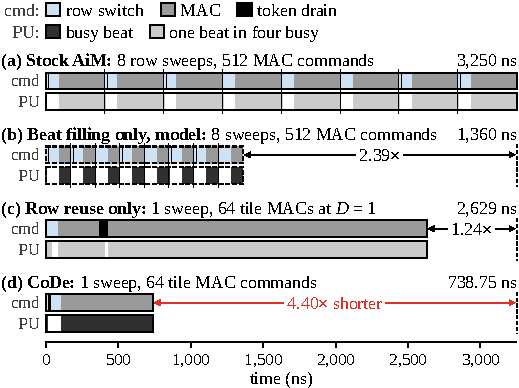
\includegraphics[width=\columnwidth]{figs/fig_sequence.pdf}
  \caption{One weight row in steady state: (a)~stock AiM; (b)~CoDe.}
  \label{fig:sequence}
\end{figure}

\subsection{Overview: One Command, Many MAC Beats}
\label{sec:design:overview}

CoDe (Command-Decoupled PIM) issues one MAC command per weight column for a tile of $V$ token vectors, and this
\emph{tile MAC} command removes both bottlenecks of Section~\ref{sec:bg:cmd}: the idle beats inside stock AiM's MAC
slots and the row-switch commands between its row sweeps. CoDe has one component for each bottleneck. \emph{Beat
filling} (Section~\ref{sec:design:beat}) runs $D$ MAC beats per column period at the PU's own clock and fills the idle
beats; \emph{row reuse} (Section~\ref{sec:design:reuse}) lets the $V$ tokens of a tile share one row sweep and pays the
sweep's row-switch commands once. Every command still obeys every DRAM timing parameter: activations, column reads and
refreshes issue exactly as in stock AiM, and only the MAC beats leave the command stream. Per token and weight column,
CoDe thus issues $1/V$ MAC commands, against one for stock AiM, $1/4$ for LP-Spec-style and one for P3-LLM-style.

Fig.~\ref{fig:sequence} follows one weight row of Llama-2-7B's q\_proj on the mobile platform through $M = 8$ tokens,
in steady state, as our simulator issues the commands. Stock AiM sweeps the row once per token: its eight row sweeps
take 3,250\,ns and 512 MAC commands, each sweep opens with its row-switch commands, and the PU computes one beat in
four of every MAC slot (Fig.~\ref{fig:sequence}a). CoDe sweeps the row once for all eight tokens in 738.75\,ns: one
row switch, then 64 tile MAC commands, each followed by eight beats over two column periods
(Fig.~\ref{fig:sequence}b). CoDe's window is 4.40$\times$ shorter than stock AiM's: beat filling (\ding{172}) cuts the
MAC slots from 2,560 to 640\,ns, and row reuse (\ding{173}) cuts the row switches from eight to one. The window leaves
out the WRGB burst that loads the next $K$ chunk's inputs into the GB once per 64 row sweeps; over the whole q\_proj
GEMM, CoDe runs 4.31$\times$ faster than stock AiM.

\subsection{Beat Filling}
\label{sec:design:beat}

Beat filling decouples the PU's MAC beats from the command stream. The PU runs its beats at its own clock,
$f_\mathrm{PU} = D / t_\mathrm{col}$, which equals CK on both platforms (Table~\ref{tab:params}), so the PU fits $D$
beats into each column period whatever the command spacing. A tile MAC holds its column in the PU for $V/D$ column
periods, and the next tile MAC issues $V/D$ periods later. The CoDe row of Fig.~\ref{fig:timeline} shows one tile of
$V = 8$ tokens at $D = 4$. The command for a column issues at $0T$; the bank holds the column for $V/D = 2$ periods
while the PU runs eight beats, one per token, each adding into that token's accumulator slot. The command for the next
column issues at $2T$, after the eight beats on the first column, and the tile's partial sums leave in one burst after
its last column. With $V = D$ the tile fills exactly one column period, and the MAC commands follow the bank's column
rate.

Beat filling raises the slot factor from stock AiM's 1/4 to 1, because every beat of a MAC slot computes for one token
of the tile. A PU with the stock multiplier count thus reaches the same 4$\times$ ceiling that LP-Spec-style reaches with
four times the multipliers. At $V = 8$ the command bus carries one MAC command every two column periods and leaves the
rest to the kernel's activations, drains and refreshes (Section~\ref{sec:eval:phone}). Two structures carry beat
filling, the weight latch that holds the column and the beat sequencer that steps the token index
(Section~\ref{sec:design:pu}). Beat filling needs a tile of at least $D$ tokens, so no design builds beat filling without
row reuse, and Section~\ref{sec:eval:server} composes beat filling alone from the model.

% float placed early (cited first in III-D): column-width schematic
\begin{figure}[t]
  \centering
  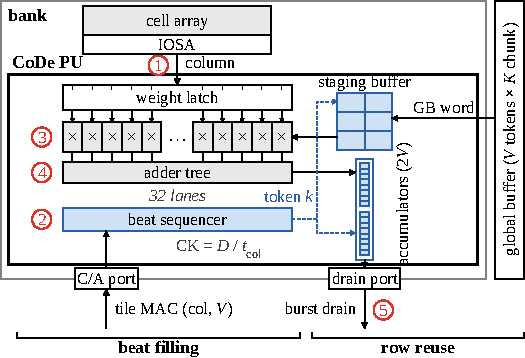
\includegraphics[width=\columnwidth]{figs/fig_tile.pdf}
  \caption{The CoDe PU inside its bank; tint marks the structures CoDe adds or sizes by $V$.}
  \label{fig:tile}
\end{figure}

\subsection{Row Reuse}
\label{sec:design:reuse}

Row reuse lets the $V$ tokens of a tile share one row sweep. The tile MACs sweep the open row's columns once for all
$V$ tokens, so the row-switch commands, two TMODs, the row's PREA and ACT16 pair and the WRMAC16, are paid once per $V$
tokens instead of once per token, and the sweep factor rises. In Fig.~\ref{fig:sequence}, CoDe's single row switch
(\ding{173}) replaces stock AiM's eight. Row reuse needs the $V$ tokens' inputs next to the PU for the whole row sweep
and $V$ partial sums per tile; the global buffer, the staging register and the accumulator file hold them
(Section~\ref{sec:design:pu}). The token load/drain commands stay per token: WRGB writes each token's input chunk into
the GB, and the burst drain reads each token's sums once per row sweep.

\subsection{Tile MAC Command and PU Microarchitecture}
\label{sec:design:pu}

\paragraph{Command set}
CoDe adds two commands to the all-bank interface of AiM-style PIM~\cite{aimjssc} and keeps every other command
(Table~\ref{tab:cmds}). The tile MAC (col, $V$) reads one column from every open bank with the stock MAC command's
timing and tells each PU to run $V$ beats on that column. The burst drain moves a tile's $V$ sums out of every PU in
one burst after the tile's last column. WRGB, TMOD, PREA, ACT16 and WRMAC16 keep their stock definitions, and of these
only the row-switch commands change their count per token.


\paragraph{Tile MAC in the PU}
Fig.~\ref{fig:tile} follows one tile MAC through the PU. The tile MAC latches the column that the bank delivers in the
weight latch (\ding{172}). The beat sequencer then steps a token index $k$ from 0 to $V-1$, one beat per CK cycle
(\ding{173}). Beat $k$ multiplies the latched weights by staging slot $k$ in the 32 lanes (\ding{174}), and the adder
tree adds the products into accumulator slot $k$ (\ding{175}). After the tile's last column, the burst drain moves the
$V$ sums out through the drain port (\ding{176}).

\paragraph{Storage}
The global buffer holds the tile's $V$ tokens for one chunk of $K$. On the mobile platform a $K$ chunk holds 2,048 INT8
inputs, 2\,KB per token, so the GB of an eight-token tile holds 16\,KB (Table~\ref{tab:params}); one WRGB burst of 512
writes of 32\,B fills it. A queue of GB words fills the staging register: on the mobile platform a three-entry queue of
512-bit words, each word packing two tokens' slices. The accumulator file holds $2V$ slots in two sets of $V$, so one
tile's sums drain from one set while the next tile accumulates into the other.

% command table (cited first in III-D): defined in III-D's right-hand column, so it renders at that column's
% top, opposite Fig. tile; generated by scripts/make_fig_sequence.py
\begin{table}[t]
  \caption{CoDe's commands, counted per token against stock AiM.}
  \label{tab:cmds}
  \centering
  \footnotesize
  \setlength{\tabcolsep}{2.5pt}
  % generated by scripts/make_fig_mapping.py (counts checked on the V = 8 trace, evaluation/dac_2x2 Sec. 2j); do not edit
\begin{tabular}{@{}l>{\raggedright\arraybackslash}p{3.2cm}lcc@{}}
\toprule
Command & Action & Unit & CoDe & Stock \\
\midrule
\emph{tile MAC} (col, $V$) & One column read at the stock MAC timing; $V$ beats on it & column & $1/V$ & 1 \\
\emph{burst drain} & A tile's $V$ sums out in one burst & row sweep & 1 & 1 \\
row switch & TMOD$\times$2, PREA, ACT16 pair, WRMAC16; unchanged & row sweep & $1/V$ & 1 \\
WRGB & GB fill; unchanged & 32\,B of input & 1 & 1 \\
\bottomrule
\end{tabular}

\end{table}

\paragraph{PU clock}
The tile keeps the PU clock within reach of a DRAM process. Beat $k$ writes accumulator slot $k$, so each slot takes one
update per tile of $V \ge D$ beats, and the add loop of each slot spans a column period or more; GDDR6-AiM~\cite{aimjssc}
interleaves two FP accumulators for the same reason, because one FP add does not reliably finish within 1\,ns in its
DRAM process. CoDe's lanes multiply integers, INT8 on the mobile platform and INT4\,$\times$\,INT8 on HBM2, narrower
operands than GDDR6-AiM's 1\,GHz BF16 lanes, and P3-LLM~\cite{p3llm} notes that its low-precision PU permits a higher
clock than HBM-PIM's. Each added structure grows with $V$, not with $D$: CoDe spends its area on storage and keeps the
stock multiplier count (Section~\ref{sec:eval:method}).

\subsection{Mapping Skinny GEMMs and Attention}
\label{sec:design:map}

% figure* (Section IV-B): defined in III-E, so it renders alone at the top of the next page, where IV-B cites it
\begin{figure*}[t]
  \centering
  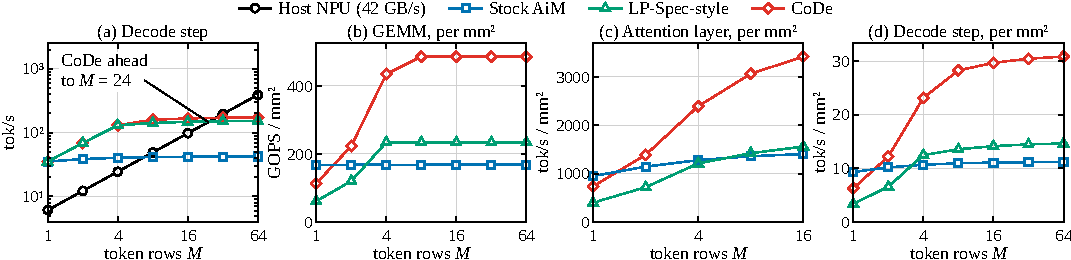
\includegraphics[width=\textwidth]{figs/fig_phone.pdf}
  \caption{Mobile platform: (a)~decode-step speed; (b)~GEMM, (c)~attention-layer and (d)~decode-step throughput per
  logic mm$^2$.}
  \label{fig:phone}
\end{figure*}

A $K \times N$ weight matrix maps as in stock AiM: the matrix's $N$ output rows spread over the banks, and each row's $K$ weights run along DRAM columns. CoDe cuts the $M$ token rows into tiles of $V$. For each tile the GB holds the tile's
activations for a chunk of $K$; every weight column of the chunk takes one tile MAC command, and the next tile repeats
the row sweep. A tile with fewer than $V$ tokens runs fewer beats on the same commands. Attention runs on the same path
with the KV cache as the weight matrix: $QK^\top$ streams the cached keys against the $M$ query rows, and $PV$ the
cached values against the $M$ rows of probabilities. Speculative decoding verifies $M$ drafted tokens against one
shared KV cache, so speculative-decoding attention is a skinny GEMM as well; a batch reads one cache per request, so batched attention
stays one GEMV per request. The host computes softmax, RoPE and normalisation between the PIM phases.
